\chapter{GIỚI THIỆU TỔNG QUAN PHẦN CỨNG VÀ LINH KIỆN}

\section{Vi điều khiển ATmega16}

\subsection{Tổng quan kiến trúc và đặc tính kỹ thuật}

ATmega16 là vi điều khiển 8-bit họ AVR của Atmel (nay thuộc Microchip Technology), sử dụng kiến trúc RISC với 131 lệnh, phần lớn thực thi trong một chu kỳ clock \cite{atmega16-datasheet}. Thông lượng xử lý có thể đạt gần 1 MIPS trên mỗi MHz, phù hợp với yêu cầu đọc cảm biến và điều khiển hiển thị của mô hình.

\begin{figure}[H]
    \centering
    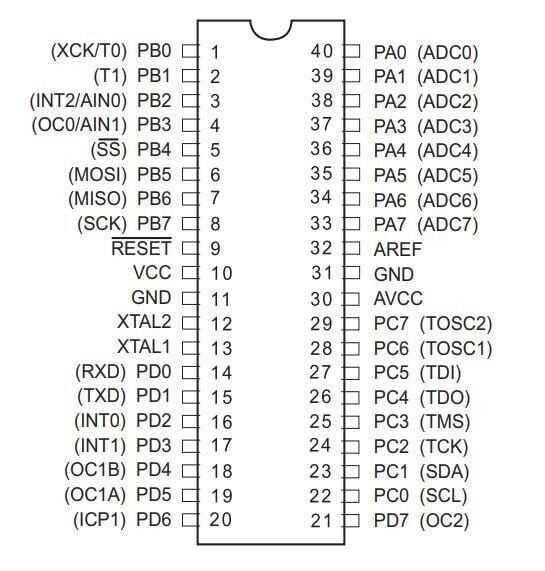
\includegraphics[width=0.75\textwidth]{atmega_sodo.png}
    \caption{Sơ đồ phân bố chân của vi điều khiển ATmega16 dạng đóng vỏ DIP-40}
    \label{fig:atmega16-pinout}
\end{figure}

Các thông số kỹ thuật then chốt của vi điều khiển ATmega16 được tổng hợp trong Bảng \ref{tab:atmega16-specs}:

\begin{table}[H]
\centering
\caption{Thông số kỹ thuật chính của vi điều khiển ATmega16}
\label{tab:atmega16-specs}
\begin{tabularx}{\textwidth}{>{\bfseries}p{5.0cm}X}
\toprule
Thông số & Giá trị định mức / Đặc tính kỹ thuật \\
\midrule
Kiến trúc CPU & 8-bit AVR RISC với 32 thanh ghi làm việc đa năng 8-bit \\
Bộ nhớ Flash chương trình & 16 Kbytes (In-System Reprogrammable Flash, độ bền 10.000 lần ghi/xóa) \\
Bộ nhớ SRAM nội & 1 Kbyte (1024 Bytes) \\
Bộ nhớ EEPROM nội & 512 Bytes (Lưu trữ dữ liệu không mất khi mất điện, độ bền 100.000 lần) \\
Tần số xung nhịp tối đa & 0 -- 16 MHz (Điện áp 4.5V -- 5.5V) \\
Số chân I/O khả trình & 32 chân chia làm 4 cổng 8-bit (PORT A, PORT B, PORT C, PORT D) \\
Bộ định thời / Bộ đếm (Timer) & 2 bộ Timer/Counter 8-bit và 1 bộ Timer/Counter 16-bit đa chức năng \\
Các kênh PWM & 4 kênh điều chế độ rộng xung phần cứng \\
Bộ chuyển đổi ADC & 8 kênh ADC 10-bit tích hợp sẵn trên PORT A \\
Giao tiếp truyền thông & USART, SPI, I2C/TWI \\
Giao diện gỡ lỗi phần cứng & Chuẩn JTAG (IEEE std. 1149.1) hỗ trợ On-Chip Debug \\
Điện áp hoạt động & 4.5V -- 5.5V đối với ATmega16 chuẩn (2.7V -- 5.5V đối với ATmega16L) \\
\bottomrule
\end{tabularx}
\end{table}

\subsection{Cấu trúc các cổng vào/ra và chức năng trong đồ án}

Vi điều khiển ATmega16 trang bị 32 chân vào ra hai chiều, được phân bổ đều cho 4 cổng ngoại vi ký hiệu từ A đến D. Mỗi cổng được kiểm soát độc lập bởi 3 thanh ghi điều khiển địa chỉ bộ nhớ:
\begin{itemize}[leftmargin=1.2cm]
    \item Thanh ghi DDRx (hướng dữ liệu): Thiết lập cấu hình hướng cho từng chân (Bit = 0: Chân là đầu vào Input; Bit = 1: Chân là đầu ra Output).
    \item Thanh ghi PORTx (dữ liệu xuất): Khi chân được thiết lập là Output, việc ghi 0 hoặc 1 vào bit tương ứng sẽ xuất điện áp mức thấp (0V) hoặc mức cao (5V). Khi chân là Input, ghi bit 1 sẽ kích hoạt điện trở kéo lên nội, ghi bit 0 sẽ đưa chân về trạng thái trở kháng cao.
    \item Thanh ghi PINx (đọc dữ liệu vào): Đọc trạng thái logic điện áp thực tế tại các chân cổng.
\end{itemize}

Trong đề tài, PA1 nối với chân dữ liệu của DHT11, PC4 -- PC7 và PD5 -- PD7 dùng cho LCD 1602, PD0 -- PD4 điều khiển 5 LED cảnh báo; bảng kết nối đầy đủ ở Bảng \ref{tab:hardware-wiring}.

\subsection{Xung nhịp hệ thống và phân tích xung đột ngoại vi JTAG}

\subsubsection{Cấu hình nguồn xung nhịp 8.0 MHz bằng Fuse Bits}
ATmega16 tích hợp sẵn mạch dao động RC nội đã hiệu chuẩn, có khả năng tạo ra các tần số xung nhịp cố định gồm 1.0 MHz, 2.0 MHz, 4.0 MHz và 8.0 MHz mà không đòi hỏi phải gắn thêm thạch anh dao động ngoài hay tụ lọc phụ trợ.

Sơ đồ kit có bố trí thạch anh ngoài \texttt{XT1} và hai tụ tải. Cấu hình phần mềm của đồ án chọn dao động RC nội 8.0 MHz, do đó không sử dụng khối thạch anh ngoài. Giá trị \texttt{F\_CPU = 8000000UL} chỉ phục vụ tính toán trễ khi biên dịch; tần số phần cứng được chọn bằng Fuse Bits. Fuse được ghi ở bước nạp chương trình bằng ProgISP (mục \ref{sec:progisp}, Hình \ref{fig:progisp-setup}) với cấu hình:
\begin{itemize}[leftmargin=1.2cm]
    \item Low Fuse Byte = \texttt{0xE4}: Thiết lập các bit \texttt{CKSEL3..0 = 0100} chọn mạch dao động RC nội 8.0 MHz, thời gian khởi động là 6 chu kỳ clock cộng trễ bổ sung điển hình 65 ms ở 5V (\texttt{SUT1..0 = 10}, Bảng 10 của datasheet).
\end{itemize}

\subsubsection{Phân tích xung đột phần cứng JTAG trên PORT C}
Mặc định khi xuất xưởng từ nhà sản xuất, bit cầu chì \texttt{JTAGEN} trên High Fuse Byte luôn được kích hoạt sẵn (\texttt{JTAGEN = 0}). Khi giao tiếp JTAG hoạt động, phần cứng vi điều khiển sẽ chiếm dụng cố định 4 chân trên cổng C:
\begin{itemize}[leftmargin=1.2cm]
    \item Chân PC2 = TCK (Test Clock)
    \item Chân PC3 = TMS (Test Mode Select)
    \item Chân PC4 = TDO (Test Data Output)
    \item Chân PC5 = TDI (Test Data Input)
\end{itemize}

Bus dữ liệu 4 bit của LCD 1602 nối vào PC4 -- PC7. Khi JTAG còn bật, hai chân PC4 và PC5 do khối gỡ lỗi điều khiển và không còn hoạt động như GPIO, nên LCD không nhận được chuỗi lệnh khởi tạo. Triệu chứng thường gặp là dòng 1 hiện toàn ô đen, dòng 2 để trống.

Để dùng PC4, PC5 cho LCD, đề tài tắt JTAG theo hai cách:
\begin{enumerate}[leftmargin=1.2cm]
    \item Tắt JTAG ở mức phần cứng: Cấu hình High Fuse Byte = \texttt{0xD9}. Tại giá trị này, bit 6 (\texttt{JTAGEN}) mang giá trị 1 (vô hiệu hóa JTAG), bit 5 (\texttt{SPIEN}) mang giá trị 0 (duy trì cổng nạp SPI để nạp code qua USBasp).
    \item Tắt JTAG ở mức phần mềm: Ghi bit \texttt{JTD} trên thanh ghi \texttt{MCUCSR} hai lần liên tiếp trong vòng 4 chu kỳ máy ngay ở đầu hàm \texttt{main()}:
    \begin{verbatim}
    MCUCSR = (1 << JTD);
    MCUCSR = (1 << JTD);
    \end{verbatim}
\end{enumerate}

\section{Mạch Kit thực hành vi điều khiển họ AVR}

Kit AVR sử dụng trong đồ án được triển khai từ sơ đồ nguyên lý do giảng viên cung cấp \cite{hust-kit-manual}. Nhóm vẽ lại sơ đồ và thiết kế PCB trên Altium Designer; bố trí linh kiện được thể hiện ở Hình \ref{fig:atmega-kit}.

\begin{figure}[H]
    \centering
    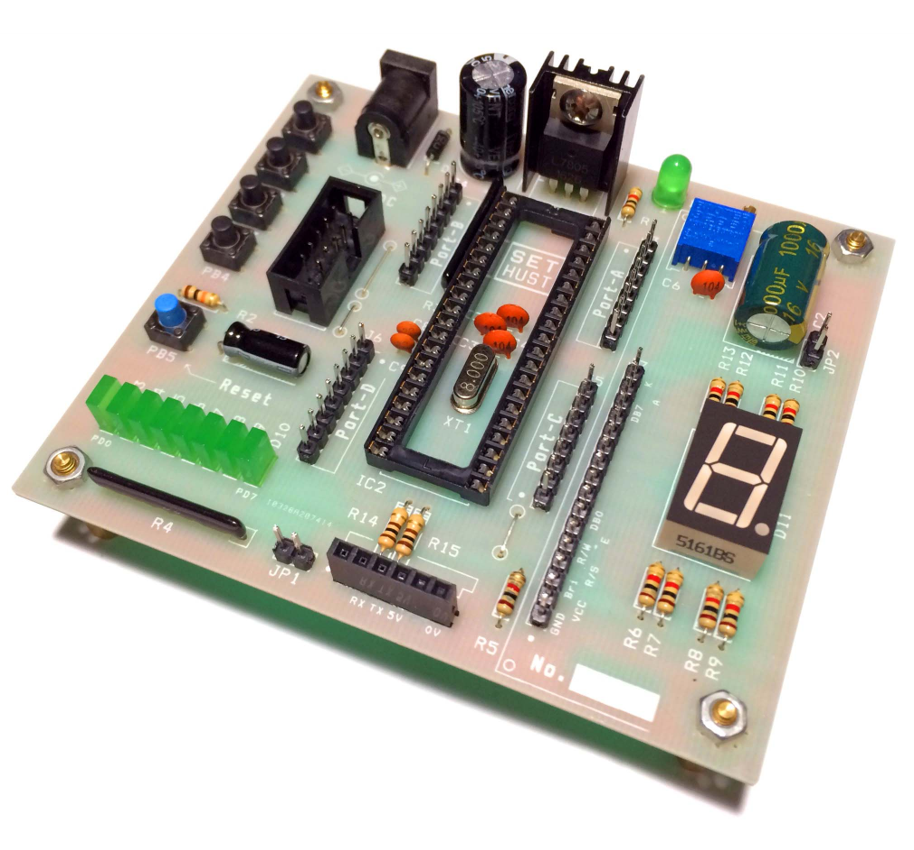
\includegraphics[width=0.78\textwidth]{atmega_kit_2d.png}
    \caption{Mô hình 3D bố trí linh kiện trên Kit phát triển vi điều khiển AVR}
    \label{fig:atmega-kit}
\end{figure}

Kit phát triển tích hợp đầy đủ các khối chức năng ngoại vi cơ bản:
\begin{enumerate}[leftmargin=1.2cm]
    \item Đế cắm vi điều khiển DIP-40: Cho phép lắp và thay thế vi điều khiển trong quá trình thực hành.
    \item Khối nguồn nuôi và ổn áp 5V: Tích hợp IC ổn áp tuyến tính LM7805 hạ áp từ nguồn Adapter ngoài DC 9V--12V, đồng thời hỗ trợ nhận nguồn 5V trực tiếp từ cổng USB qua mạch nạp USBasp, kết hợp hệ thống tụ lọc nguồn và đèn LED chỉ thị nguồn VCC.
    \item Giao diện nạp chương trình chuẩn ISP 10 chân (IDC-10): Kết nối trực tiếp với mạch nạp USBasp qua các đường tín hiệu MOSI (PB5), MISO (PB6), SCK (PB7), RESET và GND.
    \item Hàng rào cắm mở rộng J7 cho LCD 1602: Chuẩn cắm hàng đơn 16 chân tương thích với các màn hình chuẩn HD44780, tích hợp sẵn biến trở vi chỉnh VR1 dùng để điều chỉnh độ tương phản.
    \item Dàn LED đơn và phím bấm chức năng: Hệ thống 8 LED đơn nối về PORT D và ma trận nút bấm điều khiển nối về PORT B phục vụ các bài toán thực hành giao tiếp vào ra cơ bản. Đồ án dùng 5 LED trên PD0--PD4 để cảnh báo; 3 LED còn lại trên PD5--PD7 nằm chung đường với tín hiệu điều khiển LCD nên sẽ sáng theo mức logic của RW, RS, EN.
\end{enumerate}

\section{Cảm biến số nhiệt độ và độ ẩm DHT11}

\subsection{Cấu tạo và nguyên lý hoạt động}

DHT11 là cảm biến số đo nhiệt độ và độ ẩm môi trường tích hợp vi xử lý 8-bit hiệu năng cao bên trong để số hóa và hiệu chuẩn dữ liệu trước khi truyền ra ngoài \cite{dht11-datasheet}. Cấu tạo cảm biến bao gồm hai thành phần cảm nhận vật lý:
\begin{itemize}[leftmargin=1.2cm]
    \item Cảm biến độ ẩm kiểu điện trở: Sử dụng một phần tử màng polymer nhạy ẩm có các điện cực xen kẽ. Khi độ ẩm môi trường biến thiên, các phân tử hơi nước được hấp thụ vào bề mặt làm phân ly các ion dẫn, dẫn đến biến đổi điện trở của màng. Vi điều khiển 8-bit tích hợp bên trong DHT11 sẽ đo đạc sự thay đổi điện trở này và tính toán quy đổi thành giá trị độ ẩm tương đối (\%RH).
    \item Cảm biến nhiệt độ NTC: Là một điện trở nhiệt bán dẫn có hệ số nhiệt điện trở âm. Khi nhiệt độ môi trường tăng lên, điện trở của linh kiện giảm xuống theo một hàm phi tuyến được định trước. Vi điều khiển chuyển đổi giá trị điện trở này thành nhiệt độ thực tế theo thang đo độ Celsius ($^\circ\text{C}$).
\end{itemize}

\begin{table}[H]
\centering
\small
\caption{Đặc tính kỹ thuật của cảm biến số DHT11}
\label{tab:dht11-specs}
\begin{tabularx}{\textwidth}{>{\bfseries}p{5.0cm}X}
\toprule
Thông số kỹ thuật & Giá trị danh định \\
\midrule
Điện áp hoạt động & 3.0V -- 5.5V DC (theo bản tài liệu tham chiếu) \\
Dải đo nhiệt độ & $0^\circ\text{C}$ -- $50^\circ\text{C}$ \\
Độ chính xác đo nhiệt độ & $\pm 2.0^\circ\text{C}$ \\
Độ phân giải nhiệt độ & $1.0^\circ\text{C}$ (bản DHT11 trong tài liệu tham chiếu) \\
Dải đo độ ẩm & 20\% -- 90\% RH \\
Độ chính xác đo độ ẩm & $\pm 5.0\%$ RH \\
Độ phân giải độ ẩm & 1\% RH \\
Khoảng cách giữa các lần đọc & Tối thiểu 1 giây theo bản tài liệu tham chiếu; chương trình chọn trễ 2 giây mỗi vòng lặp \\
Dòng điện tiêu thụ & $0.5\text{ mA} - 2.5\text{ mA}$ khi đo; $100\text{ }\mu\text{A} - 150\text{ }\mu\text{A}$ khi chờ \\
Chuẩn giao tiếp & Aosong 1-Wire Single-Bus (Đường truyền đơn tuyến chuyên biệt) \\
\bottomrule
\end{tabularx}
\end{table}

Module sử dụng trong mô hình là loại DHT11 gắn trên PCB, đầu nối 3 chân, mã bán hàng \texttt{LK\_02463}. Mã này không xác định phiên bản chip hoặc bản datasheet. Khi đấu nối cần dựa trên nhãn VCC, DATA (hoặc S) và GND trên module, không áp dụng trực tiếp số chân của cảm biến rời 4 chân. Bảng \ref{tab:dht11-specs} dùng làm cơ sở tham chiếu cho DHT11. Chương trình hiển thị trực tiếp Byte 2 ($T_{int}$) và Byte 3 ($T_{dec}$) lên LCD, nên các giá trị $26.5^\circ\text{C}$ và $31.5^\circ\text{C}$ ghi nhận ở Chương 3 cho thấy module thực tế trả về byte thập phân khác 0, khác với mức phân giải $1^\circ\text{C}$ của bản tài liệu tham chiếu.

\subsection{Giao thức truyền thông đơn tuyến Aosong 1-Wire}
\label{sec:dht11-protocol}

\textbf{Phân định chuẩn giao thức}: Giao thức truyền thông một dây (Single-Bus) của DHT11 do nhà sản xuất Aosong thiết kế là giao thức điểm--điểm chuyên biệt, \textbf{không tương thích} với chuẩn công nghiệp Dallas/Maxim 1-Wire (vốn sử dụng mã định danh ROM 64-bit, khe thời gian do Master chủ động điều khiển và hỗ trợ kết nối đa điểm trên cùng một bus). Giao thức của DHT11 hoạt động theo nguyên tắc Master phát xung khởi động kích hoạt một lần, sau đó Slave (cảm biến) tự động phát liên tục chuỗi 40 bit dữ liệu theo các mốc thời gian quy ước.

Cảm biến DHT11 giao tiếp với vi điều khiển chỉ thông qua một chân dữ liệu DATA duy nhất. Đường tín hiệu này đòi hỏi phải có một điện trở kéo lên nguồn 5V (giá trị từ 4.7 k$\Omega$ đến 10 k$\Omega$) để duy trì mức cao khi đường truyền ở trạng thái rảnh rỗi.

Toàn bộ quy trình trao đổi dữ liệu một lần đọc (gồm 40 bit) tuân theo trình tự định thì thời gian nghiêm ngặt được mô tả dưới đây:

\subsubsection{1. Tín hiệu khởi động}
Vi điều khiển phát tín hiệu khởi động:
\begin{itemize}[leftmargin=1.2cm]
    \item MCU cấu hình chân PA1 thành Output và kéo đường bus xuống mức LOW trong thời gian tối thiểu 18 ms (trong chương trình chọn trễ an toàn là \texttt{\_delay\_ms(20)}).
    \item MCU sau đó giải phóng quyền điều khiển bus bằng cách chuyển chân PA1 sang chế độ Input và kích hoạt điện trở kéo lên nội, tạo khoảng trễ 30 $\mu$s để đường tín hiệu được kéo lên mức HIGH an toàn trước khi cảm biến bắt đầu phản hồi. Việc chuyển sang đầu vào cho phép cảm biến điều khiển đường DATA mà không bị MCU chủ động giữ mức cao.
\end{itemize}

\subsubsection{2. Tín hiệu phản hồi từ cảm biến}
Khi nhận diện được xung khởi động hợp lệ, DHT11 sẽ kéo đường bus xuống mức LOW trong khoảng 80 $\mu$s, tiếp theo kéo lên mức HIGH trong 80 $\mu$s để thông báo đã sẵn sàng truyền gói dữ liệu.

\subsubsection{3. Thu nhận và giải mã 40 bit dữ liệu}
Sau khi gửi tín hiệu phản hồi, DHT11 bắt đầu tuần tự phát ra 40 bit nhị phân (chia đều thành 5 byte). Mỗi bit dữ liệu luôn được bắt đầu bằng một xung mức LOW kéo dài cố định khoảng 50 $\mu$s. Giá trị của bit nhị phân được mã hóa dựa trên độ rộng thời gian tồn tại của xung mức HIGH tiếp theo đó:
\begin{itemize}[leftmargin=1.2cm]
    \item Bit '0': Xung mức HIGH tồn tại trong khoảng từ 26 $\mu$s đến 28 $\mu$s.
    \item Bit '1': Xung mức HIGH tồn tại kéo dài trong khoảng 70 $\mu$s.
\end{itemize}

Cách vi điều khiển phân biệt hai độ rộng xung này được trình bày ở mục \ref{sec:dht11-read}.

\subsubsection{4. Cấu trúc gói tin và cơ chế kiểm tra lỗi}
Gói dữ liệu hoàn chỉnh gồm 5 byte (40 bit) truyền đi theo thứ tự:
\begin{equation}
\begin{aligned}
    \text{Gói dữ liệu} = \{ & \text{Byte 0: } RH_{int}, \quad \text{Byte 1: } RH_{dec}, \\
                            & \text{Byte 2: } T_{int}, \quad \text{Byte 3: } T_{dec}, \quad \text{Byte 4: } Checksum \}
\end{aligned}
\end{equation}

Byte cuối cùng là byte kiểm tra lỗi Checksum được tạo bởi tổng đại số của 4 byte dữ liệu trước đó (lấy 8 bit thấp):
\begin{equation}
    Checksum_{valid} = (RH_{int} + RH_{dec} + T_{int} + T_{dec}) \ \& \ \text{0xFF}
\end{equation}

Nếu giá trị tính toán trùng khớp với Byte 4 nhận được từ cảm biến, gói dữ liệu được xác nhận là hợp lệ. Thuật toán Checksum 8-bit giúp phát hiện hiệu quả các trường hợp méo dạng xung hoặc sai lệch bit đơn lẻ trên đường truyền; tuy nhiên, phương pháp tổng kiểm tra cộng 8-bit không có khả năng sửa lỗi và không thể loại trừ hoàn toàn các lỗi đảo bit bù trừ đa điểm.

\section{Màn hình hiển thị tinh thể lỏng LCD 1602}

Màn hình LCD 1602 là mô-đun hiển thị ký tự gồm 2 hàng, mỗi hàng có khả năng hiển thị tối đa 16 ký tự ma trận điểm $5 \times 8$ pixels, sử dụng vi mạch điều khiển tiêu chuẩn công nghiệp Hitachi HD44780 \cite{hd44780-datasheet}.

\begin{table}[H]
\centering
\caption{Bảng ánh xạ kết nối chân giữa giắc J7 trên Kit, màn hình LCD 1602 và ATmega16}
\label{tab:lcd-pinout}
\begin{tabularx}{\textwidth}{c c c >{\bfseries}c X}
\toprule
Chân J7 & Chân LCD & Tên chân & Chân MCU & Chức năng kỹ thuật \\
\midrule
1 & 1 & $V_{SS}$ & GND & Cực âm nguồn nuôi (0V) \\
2 & 2 & $V_{DD}$ & VCC & Cực dương nguồn nuôi (+5V) \\
3 & 3 & $V_0$ & VR1 & Điện áp điều chỉnh độ tương phản hiển thị màn hình \\
4 & 4 & RS & PD6 & Chọn thanh ghi (0: Thanh ghi Lệnh; 1: Thanh ghi Dữ liệu) \\
5 & 5 & RW & PD5 & Chọn chiều Đọc/Ghi (0: Ghi dữ liệu vào LCD; 1: Đọc từ LCD) \\
6 & 6 & E & PD7 & Chốt xung kích hoạt (Enable Strobe, tích cực sườn âm) \\
7 -- 10 & 7 -- 10 & D0 -- D3 & PC0 -- PC3 & 4 bit dữ liệu thấp (Không dùng ở chế độ 4-bit bus) \\
11 & 11 & D4 & PC4 & Bit dữ liệu D4 \\
12 & 12 & D5 & PC5 & Bit dữ liệu D5 \\
13 & 13 & D6 & PC6 & Bit dữ liệu D6 \\
14 & 14 & D7 & PC7 & Bit dữ liệu D7 \\
15 & 15 & A (LED+) & VCC & Cực anot đèn nền \\
16 & 16 & K (LED-) & GND & Cực katot đèn nền \\
\bottomrule
\end{tabularx}
\end{table}

Để tối ưu hóa số lượng chân vi điều khiển, đồ án áp dụng chế độ truyền thông 4-bit bus:
\begin{itemize}[leftmargin=1.2cm]
    \item Vi điều khiển chỉ cần dùng 4 chân GPIO (PC4 -- PC7) nối tới các chân dữ liệu D4 -- D7 của LCD, tiết kiệm được 4 chân so với chế độ 8-bit truyền thống.
    \item Mỗi byte dữ liệu hoặc mã lệnh 8-bit sẽ được tách làm hai nửa byte: 4 bit cao được truyền trước kèm theo một xung chốt Enable trên chân PD7, tiếp theo 4 bit thấp được dịch sang và truyền kèm theo một xung chốt Enable thứ hai.
\end{itemize}

\section{Khối cảnh báo và chỉ thị LED}

Dàn 5 đèn LED cảnh báo trên Kit thí nghiệm được nối trực tiếp vào các chân từ PD0 đến PD4 của cổng D. Mạch được thiết kế theo cấu hình tích cực mức thấp (Active Low):
\begin{itemize}[leftmargin=1.2cm]
    \item Cực Anot của các đèn LED được cấp nguồn dương VCC qua mạng điện trở hạn dòng R4 và jumper JP1. Trên sơ đồ kit, R4 được ghi giá trị 10 k$\Omega$.
    \item Cực Katot của các đèn LED nối về các chân vi điều khiển PD0 -- PD4.
    \item Khi vi điều khiển xuất mức 0 (mức thấp): Dòng điện chạy từ VCC qua LED xuống chân vi điều khiển khép mạch, LED bật sáng (báo động vượt ngưỡng).
    \item Khi vi điều khiển xuất mức 1 (mức cao): Không có chênh lệch điện áp qua diode, LED tắt (trạng thái không cảnh báo quá nhiệt).
\end{itemize}
